\documentclass[a4paper,12pt]{article}
\usepackage[left=1cm,right=1cm,top=2cm,bottom=2cm]{geometry}
\usepackage{tikz}
%\usepackage{xcolor}

\definecolor{dorablue}{RGB}{41,138,191}
\definecolor{dorared}{RGB}{234,0,0}

\begin{document}

\begin{center}
	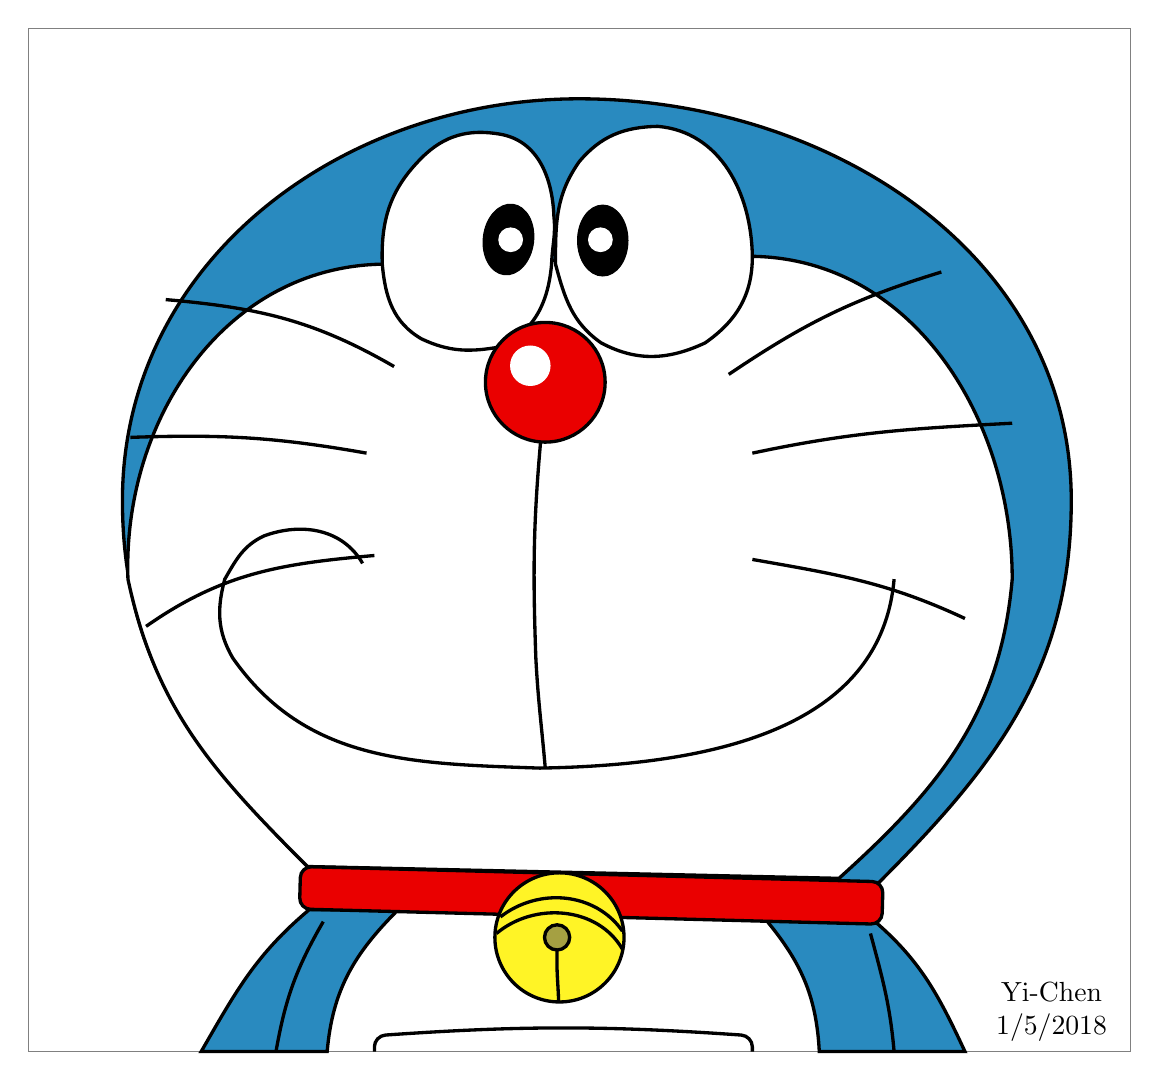
\begin{tikzpicture}
		\draw[help lines] (0,0) rectangle(14,13);

		%outfit
		\draw[fill=dorablue,very thick] (10.8,2.14) to [out=45,in=270] (13.25,7) to [out=90,in=0] (7,12.1) to [out=180,in=90] (1.2,7) to [out=270,in=135] (3.55,2.35) -- cycle;

		%face outfie
		\draw[fill=white,very thick] (10.3,2.2) to [out=42,in=265] (12.5,6) to [out=90,in=0] (9.15,10.1) -- (4.5,10) to [out=181,in=92] (1.27,6) to [out=282,in=135] (3.55,2.35) -- cycle;

		% left eye
		\draw[fill=white,very thick] (4.5,10) to [out=275,in=150] (5,9.05) to [out=335,in=190] (6,8.95) to [out=25,in=265] (6.65,10) to [out=88,in=276] (6.68,10.6) to [out=92,in=350] (6,11.65) to [out=170,in=45] (5,11.35) to [out=225,in=92] cycle;
		% right eye
		\draw[fill=white,very thick] (6.7,10) to [out=285,in=145] (7.28,9) to [out=332,in=205] (8.6,9) to [out=35,in=270] (9.2,10.1) to [out=91,in=355] (8,11.75) to [out=181,in=50] (7,11.3) to [out=235,in=90] cycle;

		% left eyeball
		\filldraw[rotate=-7] (4.8,10.98) ellipse (0.32 and 0.45);
		\filldraw[white] (6.13,10.31) circle (0.15);

		% right eyeball
		\filldraw (7.3,10.3) ellipse (0.32 and 0.45);
		\filldraw[white] (7.27,10.31) circle (0.15);

		% nose
		\draw[fill=dorared, very thick] (6.57,8.5) circle (0.76);
		\filldraw[white] (6.38,8.71) circle (0.25);
		\draw[very thick] (6.51,7.74) to [out=265,in=92] (6.45,5) to [out=273,in=95] (6.57,3.6);

		% smille
		\draw[very thick] (4.25,6.2) to [out=120,in=20] (3,6.55) to [out=205,in=60] (2.5,6)  to [out=255,in=120] (2.6,5) to [out=305,in=178] (6.5,3.6) to [out=1,in=265] (11,6);

		% beard
		\draw[very thick] (1.75,9.55) to [out=355,in=150] (4.65,8.7);
		\draw[very thick] (1.3, 7.8) to [out=2,in=170] (4.3,7.6);
		\draw[very thick] (1.5,5.4) to [out=35,in=185] (4.4,6.3);
		\draw[very thick] (8.9,8.6) to [out=34,in=197] (11.6,9.9);
		\draw[very thick] (9.2,7.6) to [out=12,in=183] (12.5,7.98);
		\draw[very thick] (9.2,6.25) to [out=350,in=155] (11.9,5.5);

		% body
		\draw[fill=dorablue,very thick] (3.57,1.8) to [out=220,in=60] (2.2,0) -- (3.8,0) to [out=85, in=225] (4.7,1.8) -- cycle;
		\draw[very thick] (3.15,0) to [out=80,in=240] (3.75,1.65);
		\draw[fill=dorablue,very thick] (9.35,1.7) to [out=310,in=93] (10.05,0) -- (11.9,0) to [out=115,in=320] (10.7,1.7);
		\draw[very thick] (10.7,1.5) to [out=285,in=95] (11,0);

		% red neck
		\draw[fill=dorared, very thick, rotate=-1.5, rounded corners=4pt] (3.4,1.9) rectangle (10.8,2.44);

		% Bell
		\draw[fill=yellow!85,very thick] (6.75,1.45) circle (0.82);
		\draw[fill=yellow!60!black,very thick] (6.72,1.45) circle (0.16);
		\draw[very thick] (6.72,1.29) to [out=268,in=92] (6.74,0.63);
		\draw[very thick] (6,1.71) to [out=38,in=125] (7.55,1.53);
		\draw[very thick] (5.95,1.5) to [out=40,in=120] (7.55,1.3);

		% pocket
		\draw[very thick, rounded corners=4pt] (4.4,0) -- (4.4,0.2) to [out=4,in=176] (9.2,0.2) -- (9.2,0);

		% sign
		\draw (13,0.5) node(a) [align=center] {Yi-Chen\\1/5/2018};
	\end{tikzpicture}
\end{center}

\end{document}
